\externaldocument{../7/chapter_implementation}
\externaldocument{../6/chapter_algorithm}
\startchapter{Modeling}
\label{chapter:Mod}
The modeling aims to model the communication between two software in the perspective of dual-trace analysis. It focuses on describing what information about the communication would be captured and how that information organized in the dual-trace. The model did not cover all communication methods in the real world, but gives a general structure of the communication in the dual-trace as well as the analysis pattern of the communication. Some communication methods are leveraged in this model to give a more concrete view of the model and guideline for further investigation of other communication methods which are not covered in this work.

In this section, I define the communications between two software. Meanwhile, I list and categorize the communication methods which will be the instances of this model. After that, I present the communication model for the dual-traces analysis. This model includes two levels. The first level is the model of the general stages for all communication methods. They are 1. channel opening stage, 2. data transfer stage and 3. channel close stage. The second level models give the idea of how to investigate the patterns of the communication stages defined in the first level by modeling the stages for the selected communication methods. The modeling idea and concepts can be reused for those ones not covered in this work. Only channel open stage and data transfer stage are explored since the channel close stage is very straightforward.

This model is the guideline of what information of communication can and should be retrieved from the dual-trace for interacting software, and how they would be reconstructed and presented to the users. The second level models are also essential for the design of the communication channel identification algorithms and communication event synchronization algorithms.

\section{Communication of Two Applications}   
The communication defined in this work is data transfer activities between two running software through a specific channel. Some collaborative activities between the software such Remote procedure call is out of the scope of this research. Communication among multiple software(more than two) is not discussed in this work.

In general, these data sharing communications can be divided into two main categories: inter-process communication and network communication. There are various communication methods in both of these two categories. Table\ref{methodsInCategories} lists those ones investigated by this research. 

% Please add the following required packages to your document preamble:
% \usepackage{booktabs}


\begin{table}[H]
\centering
\caption{Communication Methods Discussed in This Work}
\label{methodsInCategories}
\begin{tabular}{|l|l|l|}
 \hline
 &  \textbf{Inter-Process}& \textbf{Network}\\
 \hline
\multirow{2}{*}{{\textbf{Methods}}} & Named Pipes & TCP   \\
 \cline{2-3}
 & Message Queue &  UDP \\
 \hline
\end{tabular}
\end{table}


\section{First Level Communication Model: General Model}   
The general model describes how a full communication happens and is generalizable for all communication. After the illustration of the model, I instantiate this model to some communication methods in Windows APIs. Windows API functions called to consist a full communication on each endpoint are listed separately for communication methods. These function call lists are the concerned information from the dual-trace in the analysis.
\subsection{Modelling}
Before describing the model, I would like to define the terms which are being used in the model
Terms:\\
\textbf{endpoint:}\\
A software or application at which data are sent or received (or both).\\
\textbf{channel:}\\
A conduit connected two endpoints through  which data can be sent and received\\
\textbf{send:}\\
One or more function calls to send a truck of data from one endpoint to the other through  the channel.\\
\textbf{receive:}\\
One or more function calls to receive a truck of data at one endpoint from the other through the channel.\\

The general communication model defines a full communication. It consists of three stages
and two endpoints which transferring data to each other. These three stages are 1. channel opening
stage, 2. data transfer stage and 3. channel close stage. Both of these two communicating endpoints
open or connect to the communication channel before they start the data transfer and close or disconnect from the channel after finishing the data transfer. The data transfer should happen in between of the channel open and the channel close.

Figure 3.1 illustrates the general communication model indicating how communications happen
between two endpoints. In the channel open stage, each endpoint needs to call one or multiple
channel open/connection functions, depending on the types of the channel endpoints(server
or client endpoint), different functions might be called. In the data transfer stage, data is being sent into the channel in one endpoint and received in the other endpoint. Both endpoints can be senders and receivers throughout the communication. Same as channel open stage, in the channel
close stage, one or multiple functions might be called by both endpoints to ensure a proper resource release and disconnection from the channel.

The channel can be reopened again to start new communications after the close stage. However,
the reopened channel will be treated as a new communication cycle with its own stages. From the
trace analysis point of view, function calls of all stages in the communications are not mandatory
being captured or happen. However channel open stage is necessary for the identification of a
channel.

\begin{figure}[H]
\centerline{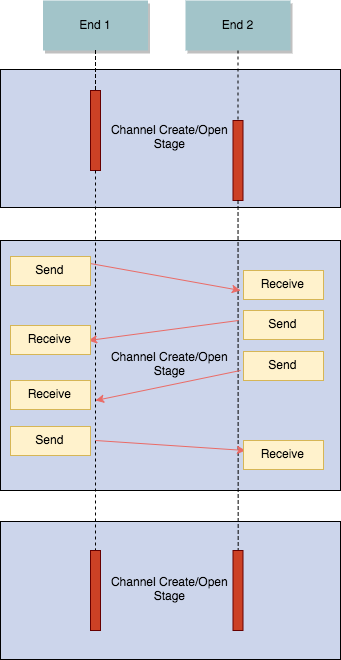
\includegraphics[scale=0.55]{Figures/communicationhappen}}
 \caption{General Communication Model}
\label{communicationhappen}
\end{figure}

\subsection{Model Instantiation}
I reviewed the Windows APIs of some communication methods. Windows API is very sophisticated
and multiple solutions are provided by windows to fulfill similar communication methods.
Windows application developers can choose what API set they want to use in their solutions. It’s
impossible to enumerate all the communication methods and all API combinations for each communication method. I only leveraged some communication methods. 

For each communication method, a function list is provided for reference. However, this function list should not be considered as the only combination or solution for each communication method. With the understanding of the model, it should be fairly easy to draw out lists for other
communication methods or other API set for the same communication methods. Moreover, the
instances of this model only demonstrate Windows C++ APIs. This model may be generalizable
to other operating systems with the effort of understanding the APIs of those operating system.

In the following subsections, Windows APIs with function names, essential parameters and
registers which holding those parameters are listed for the four investigated communication methods. These functions APIs are those ones supported in most Windows operating systems, such as
Windows 8, Window 7. The registers for the parameters are concluded according to the Windows
calling convention and can change over time.

These lists can be examples and references for the users of the implementation when they need
to generate their own communication methods setting. The user can use their own concerned API
list for the dual-trace analysis of different communication methods by putting the function lists
in JSON format as the setting. More detail of the communication methods setting will be discussed in Section \ref{chapter:newsol}, when I discuss the implementation of communication analysis of the dual-trace.

\subsubsection{Named Pipes}
In this section, I describes what is a Named Pipe channel and how it works briefly. And then I apply it to the general communication model by matching all the stages with the windows calling functions.

A named pipe is a communication method for the pipe server and one or more pipe clients. The pipe has a name, can be one-way or duplex. Both the server and client can read or write into the pipe.\cite{WinNamedpipe} In here we only consider one server versus one client communication. One server to multiple clients scenario can always be divided into multiple server/client communications thanks to the characteristic that each client/server communication has a separate conduit. The server and client are endpoints in the model. We call the server "server endpoint" while the client "client endpoint". The server endpoint and client endpoint of a named pipe share the same pipe name, but each endpoint has its own buffers and handles. 

A named pipe server is responsible for the creation of the pipe, while clients can connect to the pipe after it created. The creation and connection of a named pipe will return the handle ID of that pipe. As we mentioned before, each client or server endpoint has its own handles, so the returned handle Ids of the pipe creation function of the server and pipe connection function from each client are different. These handler Ids will be used later when data are being sent or received to specify a pipe.

There are two modes for data transfer in the named pipe communication method, synchronous and asynchronous.  Modes affect the functions used to complete the send and receive operation as well as the operation of the functions. I list the related functions for both synchronous mode and asynchronous mode. The create channel functions for both modes are the same but with different input parameters. The functions for send and receive message are also the same for both cases. However, the operation of the send and receive functions are different for the different mode. In addition, an extra function \textit{GetOverlappedResult} is being called to check if the sending or receiving operation finish, the output message will be stored in the overlap structure whose memory address saved in the function's output parameter Overlap Structure Address. Table\ref{synfunctions} lists the necessary functions for synchronous mode while Table\ref{asynfunctions} lists the necessary functions for the asynchronous mode for a full communication.

    \begin{table}[H]
        \centering
        \caption{Function APIs for Synchronous Named Pipe}
        \label{synfunctions}
        \begin{tabular}{|l|l|l|l|l|}
            \hline
             \multirow{2}{*}{\textbf{Stage}} &
               \multicolumn{2}{c|}{\textbf{Server Endpoint}} &
               \multicolumn{2}{c|}{\textbf{Client Endpoint}} \\
             \cline{2-5}
              & \textbf{Function}& \textbf{Parameters} & \textbf{Function} & \textbf{Parameters}  \\
             \hline
             \multirow{2}{*}{{\textbf{Channel Open}}}
             &\multirow{2}{*}{{CreateNamedPipe}} &  RAX: File Handler & \multirow{2}{*}{CreateFile} &  RAX: File Handler\\
              \cline{3-3} \cline{5-5}
             &&  RCX: File Name &  &  RCX: File Name\\
            \hline
             \multirow{6}{*}{{\textbf{Data Transfer}}}
             &\multirow{3}{*}{WriteFile} &  RCX: File Handle & \multirow{3}{*}{WriteFile} &  RCX: File Handle\\
              \cline{3-3} \cline{5-5}
             &&  RDX: Buffer Address &  &  RDX: Buffer Address\\
                           \cline{3-3} \cline{5-5}
             & &  R9: Message Length &  &  R9: Message Length\\
            \cline{2-5}
             & \multirow{3}{*}{ReadFile}&  RCX: File Handle & \multirow{3}{*}{ReadFile} &  RCX: File Handle\\
              \cline{3-3} \cline{5-5}
              &&  RDX: Buffer Address &  &  RDX: Buffer Address\\
                           \cline{3-3} \cline{5-5}
             & &  R9: Message Length &  &  R9: Message Length\\
            \hline
           {{\textbf{Channel Close}}}
             &{CloseHandle} & {RCX: File Handler} & {CloseHandle} & {RCX: File Handler}\\
            \hline
        \end{tabular}
    \end{table}

    \begin{table}[H]
        \centering
        \caption{Function APIs for Asynchronous Named Pipe}
        \label{asynfunctions}
        \begin{tabular}{|l|l|l|l|l|}
            \hline
             \multirow{2}{*}{\textbf{Stage}} &
               \multicolumn{2}{c|}{\textbf{Server Endpoint}} &
               \multicolumn{2}{c|}{\textbf{Client Endpoint}} \\
             \cline{2-5}
              & \textbf{Function}& \textbf{Parameters} & \textbf{Function} & \textbf{Parameters}  \\
             \hline
             \multirow{2}{*}{{\textbf{Channel Open}}}
             &\multirow{2}{*}{{CreateNamedPipe}} &  RAX: File Handler & \multirow{2}{*}{CreateFile} &  RAX: File Handle\\
              \cline{3-3} \cline{5-5}
             &&  RCX: File Name &  &  RCX: File Name\\
            \hline
             \multirow{8}{*}{{\textbf{Data Transfer}}}
             &\multirow{3}{*}{WriteFile} &  RCX: File Handle & \multirow{3}{*}{WriteFile} &  RCX: File Handle\\
              \cline{3-3} \cline{5-5}
             &&  RDX: Buffer Address &  &  RDX: Buffer Address\\
                           \cline{3-3} \cline{5-5}
             & &  R9: Message Length &  &  R9: Message Length\\
            \cline{2-5} 

             & \multirow{3}{*}{ReadFile}&  RAX: File Handle & \multirow{3}{*}{ReadFile} &  RCX: File Handle\\
              \cline{3-3} \cline{5-5}
              &&  RDX: Buffer Address &  &  RDX: Buffer Address\\
                           \cline{3-3} \cline{5-5}
             & &  R9: Message Length &  &  R9: Message Length\\
              \cline{2-5} 
             & \multirow{2}{*}{GetOverlapped-}&  RCX: File Handler & \multirow{2}{*}{GetOverlapped-} &  RCX: File Handler\\
              \cline{3-3} \cline{5-5}
             &  \multirow{2}{*}{Result} &  RDX:  Overlap  &  \multirow{2}{*}{Result }&  RDX:  Overlap \\
              &  &  Structure address &  &  Structure Address\\
            \hline                       
            \textbf{Channel Close}
             &{CloseHandle} &{RCX: File Handler} & {CloseHandle} &  {RCX: File Handler}\\
            \hline
        \end{tabular}
    \end{table}
    


\subsubsection{Message Queue}
In this section, I describes what is a Message Queue channel and how it works briefly. And then I apply it to the general communication model by matching all the stages with the windows calling functions.

Message Queuing (MSMQ) is a communication method to allow applications which are running at different times across heterogeneous networks and systems that may be temporarily offline can still communicate with each other. Messages are sent to and read from queues by applications. Multiple sending applications can send messages to and multiple receiving applications can read messages from one queue. \cite{redkar2004pro} The applications are the endpoints of the communication. In this work, only one sending application versus one receiving application case is considered. Multiple senders to multiples receiver scenario can always be divided into multiple sender/receiver. Both endpoints of a communication can send to and receive from the channel.

The endpoints of the communication can create the queue or use the existing one. However, both of them have to open the queue before they access it. The handle ID returned by the open queue function will be used later on when messages are being sent or received to identify the queue.

Similar to Named Pipe, Message Queue also has two modes, synchronous and asynchronous. Moreover, the asynchronous mode further divides into two operations, one with callback function while the other without. If with the callback function, the callback function would be called when the send or receive operations finish. If without callback function, the general function \textit{MQGetOverlappedResult} should be called by the endpoint to check if the message sending or receiving operation finish, the output message will be stored in the overlap structure whose memory address saved in the function's output parameter Overlap Structure Address. Table\ref{msmqsynfunctions} lists the necessary functions for synchronous mode while Table\ref{msmqasynfunctionscallback} and Table\ref{msmqasynfunctions} list the necessary functions for the asynchronous mode with and without callback for a full communication. 

    \begin{table}[H]
        \centering
        \caption{Function APIs for Synchronous MSMQ}
        \label{msmqsynfunctions}
        \begin{tabular}{|l|l|l|}
            \hline
             \textbf{Stage} & \textbf{Function}& \textbf{Parameters}  \\
             \hline
             \multirow{2}{*}{{\textbf{Channel Open}}}
             &\multirow{2}{*}{{MQOpenQueue}} &  RAX: Queue Handler\\
              \cline{3-3} 
             & &  RCX: Queue Format Name\\
            \hline
             \multirow{4}{*}{{\textbf{Data Transfer}}}
             &\multirow{2}{*}{MQSendMessage} &  RCX: Queue Handle \\
              \cline{3-3} 
             &&  RDX: Message description structure Address \\
            \cline{2-3}
             & \multirow{2}{*}{MQReceiveMessage}&  RCX: Queue Handle \\
              \cline{3-3} 
              &&  R9: Message description structure Address \\
            \hline
            \textbf{Channel Close} &MQCloseQueue & RCX: Queue Handler \\
            \hline
        \end{tabular}
    \end{table}


    \begin{table}[H]
        \centering
        \caption{Function APIs for Asynchronous MSMQ with Callback}
        \label{msmqasynfunctionscallback}
        \begin{tabular}{|l|l|l|}
            \hline
             \textbf{Stage} & \textbf{Function}& \textbf{Parameters}  \\
             \hline
             \multirow{2}{*}{{\textbf{Channel Open}}}
             &\multirow{2}{*}{{MQOpenQueue}} &  RAX: Queue Handler\\
              \cline{3-3} 
             & &  RCX: Queue Format Name\\
            \hline
             \multirow{5}{*}{\textbf{Data Transfer}}
             &\multirow{2}{*}{MQSendMessage} &  RCX: Queue Handle \\
              \cline{3-3} 
             &&  RDX: Message description structure Address \\
            \cline{2-3}
             & \multirow{2}{*}{MQReceiveMessage}&  RCX: Queue Handle \\
              \cline{3-3} 
              &&  R9: Message description structure Address \\
                            \cline{2-3} 
              &CallbackFuncName&  Parameters for the callback function. \\
            \hline
            \textbf{Channel Close} &MQCloseQueue & RCX: Queue Handler \\
            \hline
        \end{tabular}
    \end{table}



    \begin{table}[H]
        \centering
        \caption{Function APIs for Asynchronous MSMQ without Callback}
        \label{msmqasynfunctions}
        \begin{tabular}{|l|l|l|}
            \hline
             \textbf{Stage} & \textbf{Function}& \textbf{Parameters}  \\
             \hline
             \multirow{2}{*}{{\textbf{Channel Open}}}
             &\multirow{2}{*}{{MQOpenQueue}} &  RAX: Queue Handler\\
              \cline{3-3} 
             & &  RCX: Queue Format Name\\
            \hline
             \multirow{5}{*}{{\textbf{Data Transfer}}}
             &\multirow{2}{*}{MQSendMessage} &  RCX: Queue Handle \\
              \cline{3-3} 
             &&  RDX: Message description structure Address \\
            \cline{2-3}
             & \multirow{2}{*}{MQReceiveMessage}&  RCX: Queue Handle \\
              \cline{3-3} 
              &&  R9: Message description structure Address \\
                          \cline{2-3}
                          
              & MQGetOverlappedResult &  RCX: Overlap Structure address  \\
            \hline
            \textbf{Channel Close} &MQCloseQueue & RCX: Queue Handler \\
            \hline
        \end{tabular}
    \end{table}
    
\subsubsection{TCP and UDP}
In this section, I describes what is a TCP and UDP channel briefly. And then I apply it to the general communication model by matching all the stages with the windows calling functions.

TCP and UDP are the most fundamental transport methods in computer networking. TCP is a reliable transport method while UDP is not. In Windows programming, these two methods shared the same set of APIs regardless the input parameter and operation behavior is different. In Windows socket solution, one of the two endpoints is the server while the other one is the client. The server opens its socket and listens to the connection from clients. The client connects to the server after opening its own socket. 

Table \ref{tcpupdfunctions} lists the necessary functions consist a UDP or TCP full communication. For the channel opening, the function \textit{socket} should be called on both endpoints. The sever endpoint call the function \textit{bind} to bind to its local service address and port. Then the server endpoint calls the function  \textit{accept} to accept the connection from the clients. The client will call the function \textit{connect} to connect to the server. When the function \textit{accept} return successfully, a new socket handle will return for further data transfer. During the channel open stage, server endpoint has two socket handles, the first one is used to listen to the connection from the client, while the second one is created for real data transfer.
     \begin{table}[H]
        \centering
        \caption{Function APIs for TCP and UDP}
        \label{tcpupdfunctions}
        \begin{tabular}{|l|l|l|l|l|}
            \hline
             \multirow{2}{*}{\textbf{Stage}} &
               \multicolumn{2}{c|}{\textbf{Server Endpoint}} &
               \multicolumn{2}{c|}{\textbf{Client Endpoint}} \\
             \cline{2-5}
              & \textbf{Function}& \textbf{Parameters} & \textbf{Function} & \textbf{Parameters}  \\
             \hline
             \multirow{6}{*}{{\textbf{Channel Open}}}
             &socket&  RAX: Socket Handle & socket &  RAX: Socket Handle\\
              \cline{2-5}
              &\multirow{2}{*}{{bind}} &  RCX: Socket Handle & \multirow{2}{*}{connect} &  RCX: Socket Handle\\
              \cline{3-3} \cline{5-5}
             &&  RDX: Server Address $\&$ Port &  &  RDX: Server Address $\&$ Port\\
              \cline{2-5}
             &\multirow{3}{*}{{accept}} &  RAX: New Socket Handle && \\
              \cline{3-3} 
             &&  RCX:  Socket Handle &  & \\
             \cline{3-3} 
             &&  RDX: Client Address $\&$ Port &  &  \\
            \hline
             \multirow{4}{*}{{\textbf{Data Transfer}}}
             &\multirow{2}{*}{send} &  RCX: New Socket Handle & \multirow{2}{*}{send} &  RCX: Socket Handle\\
              \cline{3-3} \cline{5-5}
             &&  RDX: Buffer Address &  &  RDX: Buffer Address\\
            \cline{2-5}
             & \multirow{2}{*}{recv}&  RCX: New Socket Handle & \multirow{2}{*}{recv} &  RCX: Socket Handle\\
              \cline{3-3} \cline{5-5}
              &&  RDX: Buffer Address &  &  RDX: Buffer Address\\
            \hline
          {{\textbf{Channel Close}}}&
            {closesocket} & {RCX: New Socket Handle} &{closesocket} & {RCX: Socket Handle}\\
            \hline
        \end{tabular}
    \end{table} 
    
\section{Second Level Communication Model: Channel Open Model for Individual Communication Method}    
This section exemplifies the channel open model for the individual communication methods. This model describes how the channels are set up for communication of different method. Based on the opening process, two channel open models are depicted, one for Named pipe and Message Queue, the other for TCP and UDP. The channel identification algorithms developed in Section \ref{chapter:alo} are based on these two models.
\subsection{Model for Named Pipe and Message Queue}
In this model, the channel is already existed or created by one endpoint before the other can connect to it. So that the channel opening process is only two endpoints connect to the channel. The channel creation can happen at the same time with the channel open, but it will be treat the same as the existed channel in this model. Figure\ref{channelopen1} shows the channel set up model for Named Pipe and Message Queue.

\begin{figure}[H]
\centerline{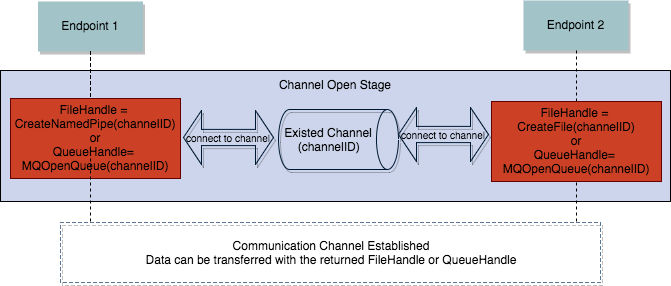
\includegraphics[scale=0.55]{Figures/channelopen1}}
 \caption{Channel Open Model for  for Named Pipes and Message Queue}
\label{channelopen1}
\end{figure}

\subsection{Model TCP and UDP}
In this model, the channel is set up by both of the endpoints. Each endpoint has to create its
own socket. After the sockets are created, the server endpoint binds the socket to it service address and port. The client endpoint connects to the service. Server endpoint accepts the client connection and generates a new data transfer socket for data transfer with this connected client. After all these operations are performed successfully, the channel is established and the data transfer can start. Figure\ref{channelopen2} shows the channel set up the model for TCP and UDP.

\begin{figure}[H]
\centerline{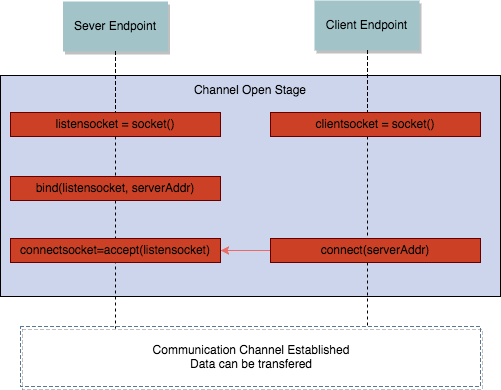
\includegraphics[scale=0.55]{Figures/channelopen2}}
 \caption{Channel Open Model for TCP and UDP}
\label{channelopen2}
\end{figure}

\section{Second Level Communication Model: Data Transfer Model for Individual Communication Method}
The four communication methods in this work all have its own properties in the perspective of data
transfer. In this section, I summarize the elemental characteristics of each communication method.
Furthermore, data transfer models for each communication method were designed respectively regarding to their characteristics. The data transfer scenarios are covered in the
models. The models in this section are fundamental for the design for communication event synchronization algorithms. The detail of these algorithms will be discussed in Section \ref{chapter:alo}.
\subsection{Named Pipe}
The basic data transfer characteristics of Named Pipe are:
\begin{itemize}
  \item Bytes received in order
  \item Bytes sent as a whole trunk can be received in segments
  \item Only the last trunk can be lost
\end{itemize}
Based on these characteristics, the data transfer model of it can be summarized in Figure\ref{namedpipe}. 
\begin{figure}[H]
\centerline{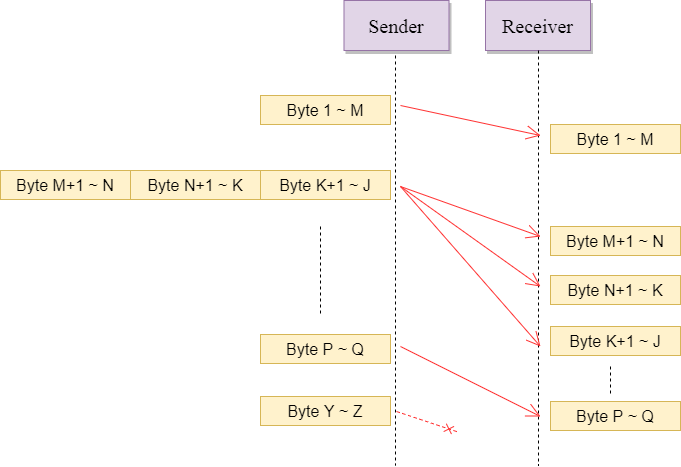
\includegraphics[scale=0.48]{Figures/namedpipe}}
\caption{Data Transfer Model for Named Pipe}
\label{namedpipe}
\end{figure}

\subsection{Message Queue}
The basic data transfer characteristics of Message Queue are:
\begin{itemize}
  \item Bytes sent in packet and received in packet, no bytes reorganized
  \item Packets can lost
  \item Packets received in order
\end{itemize}
Based on these characteristics, the data transfer model of it can be summarized in Figure\ref{msmq}.
\begin{figure}[H]
\centerline{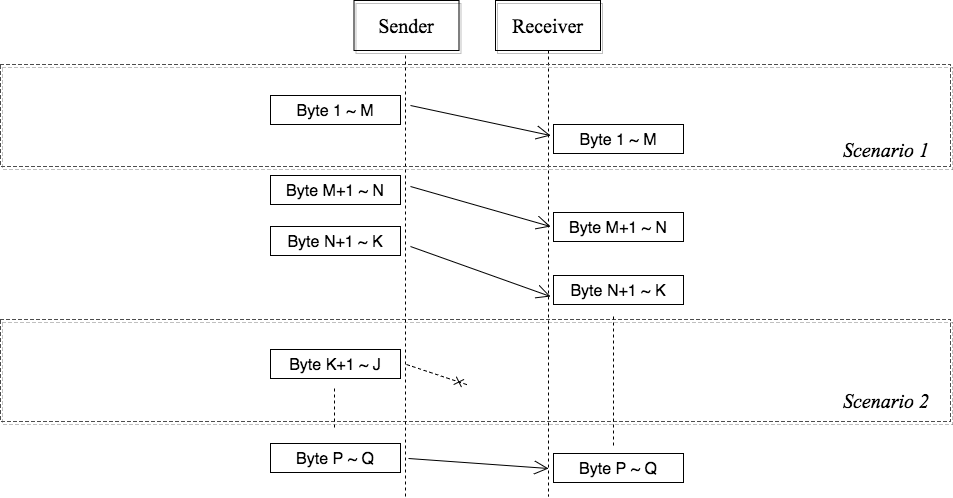
\includegraphics[scale=0.48]{Figures/msmq}}
\caption{Data Transfer Model for Message Queue}
\label{msmq}
\end{figure}

\subsection{TCP}
The basic data transfer characteristics of TCP are:
\begin{itemize}
  \item Bytes received in order
  \item No data lost
  \item Sender window size is different from receiver's window size, so packets can be re-segmented
\end{itemize}
Based on these characteristics, the data transfer model of it can be summarized in Figure\ref{tcp}.
\begin{figure}[H]
\centerline{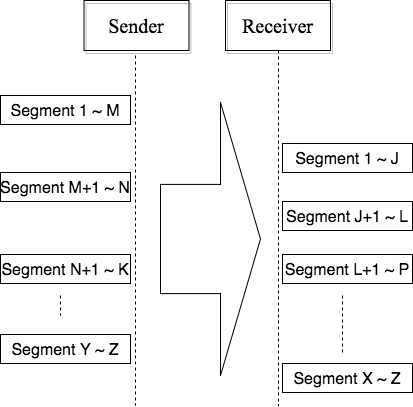
\includegraphics[scale=0.48]{Figures/tcp}}
 \caption{Data Transfer Model for TCP}
\label{tcp}
\end{figure}

\subsection{UDP}
The basic data transfer characteristics of UDP are:
\begin{itemize}
  \item Bytes sent in packet and received in packet, no re-segmentation
  \item Packets can lost
  \item Packets can arrive receiver out of order
\end{itemize}
Based on these characteristics, the data transfer model of it can be summarized in Figure\ref{upd}.
\begin{figure}[H]
\centerline{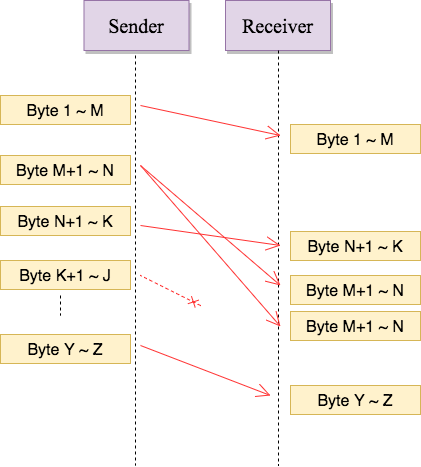
\includegraphics[scale=0.48]{Figures/udp}}
 \caption{Data Transfer Model for UDP}
\label{upd}
\end{figure}

